%%******************************************************************************
%% SECTION - Financeiro
%%******************************************************************************
\section{Financeiro}
\label{financeiro}

O relat�rio financeiro aqui apresentado t�m como objetivo demonstrar o que foi estimado no in�cio do projeto, o que foi at� o momento executado e a previs�o atual do desenbolso necess�rio at� o fim do projeto, fornecendo uma vis�o global do plano financeiro do projeto. Logo, as informa��es contidas neste  relat�rio ser�o diferentes das informa��es contidas no relat�rio financeiro de presta��o de contas, o qual detalha apenas os lan�amentos realizados na conta do projeto at� a data de fechamento do m�s. Por favor, notar que existem itens detalhados como executados neste relat�rio que n�o estar�o presentes na presta��o de contas. Isto ocorre devido a defasagem de tempo entre a decis�o de comprar o item e a data de pagamento da nota fiscal. Por mais, todos as informa��es presentes em ambos os relat�rios dever�o ser consistentes e em caso de inconsist�ncia o valor relatado no relat�rio de presta��o de contas dever ser considerado como o correto.

\subsection{Desembolso}

\begin{center}
  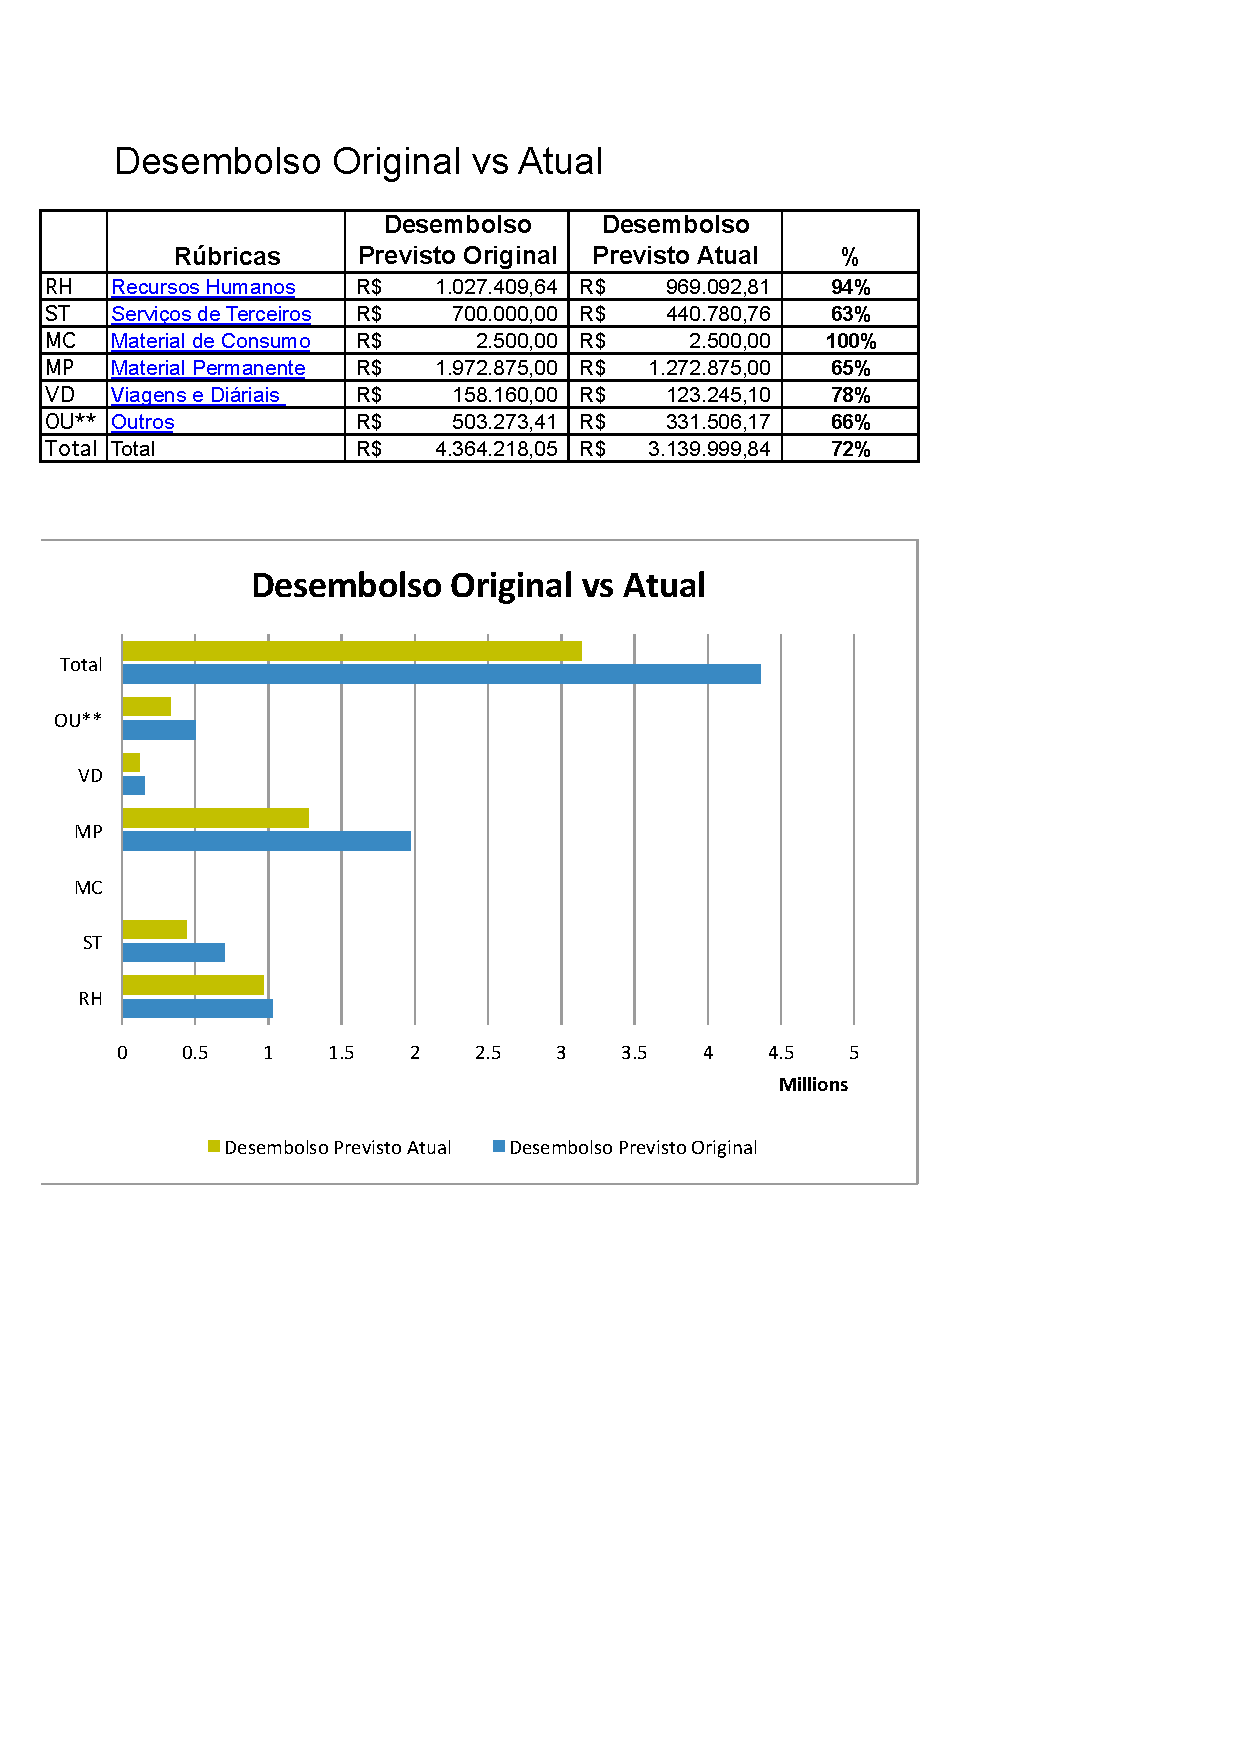
\includegraphics[width=\textwidth]{figs/financeiro/ROSA_Cronograma_Fisico_Financeiro_05_26_2014_Desenbolso.pdf}
\end{center}

\subsection{Recursos humanos}

\begin{center}
  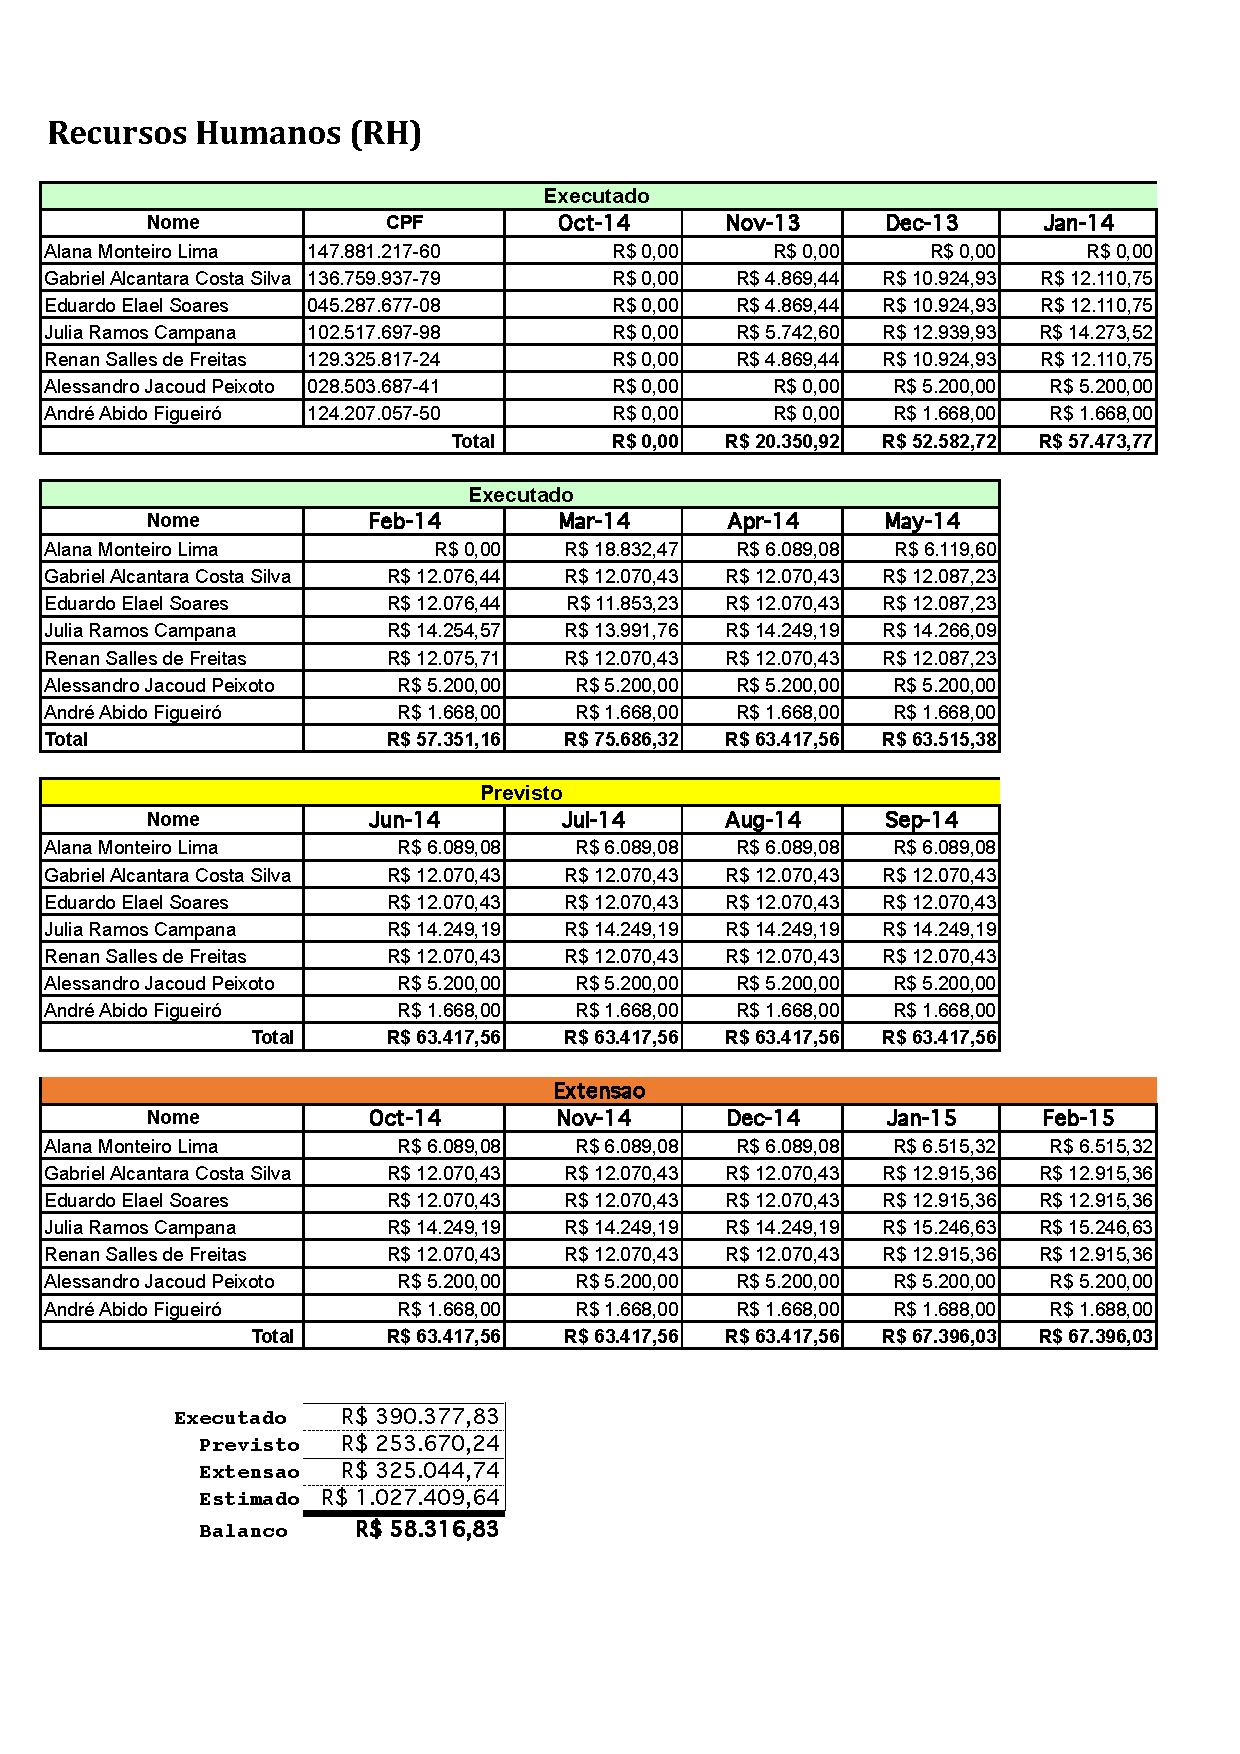
\includegraphics[width=1\columnwidth]{figs/financeiro/ROSA_Cronograma_Fisico_Financeiro_05_26_2014_RH.pdf}
\end{center}

\subsection{Servi�os de terceiros}

\begin{center}
  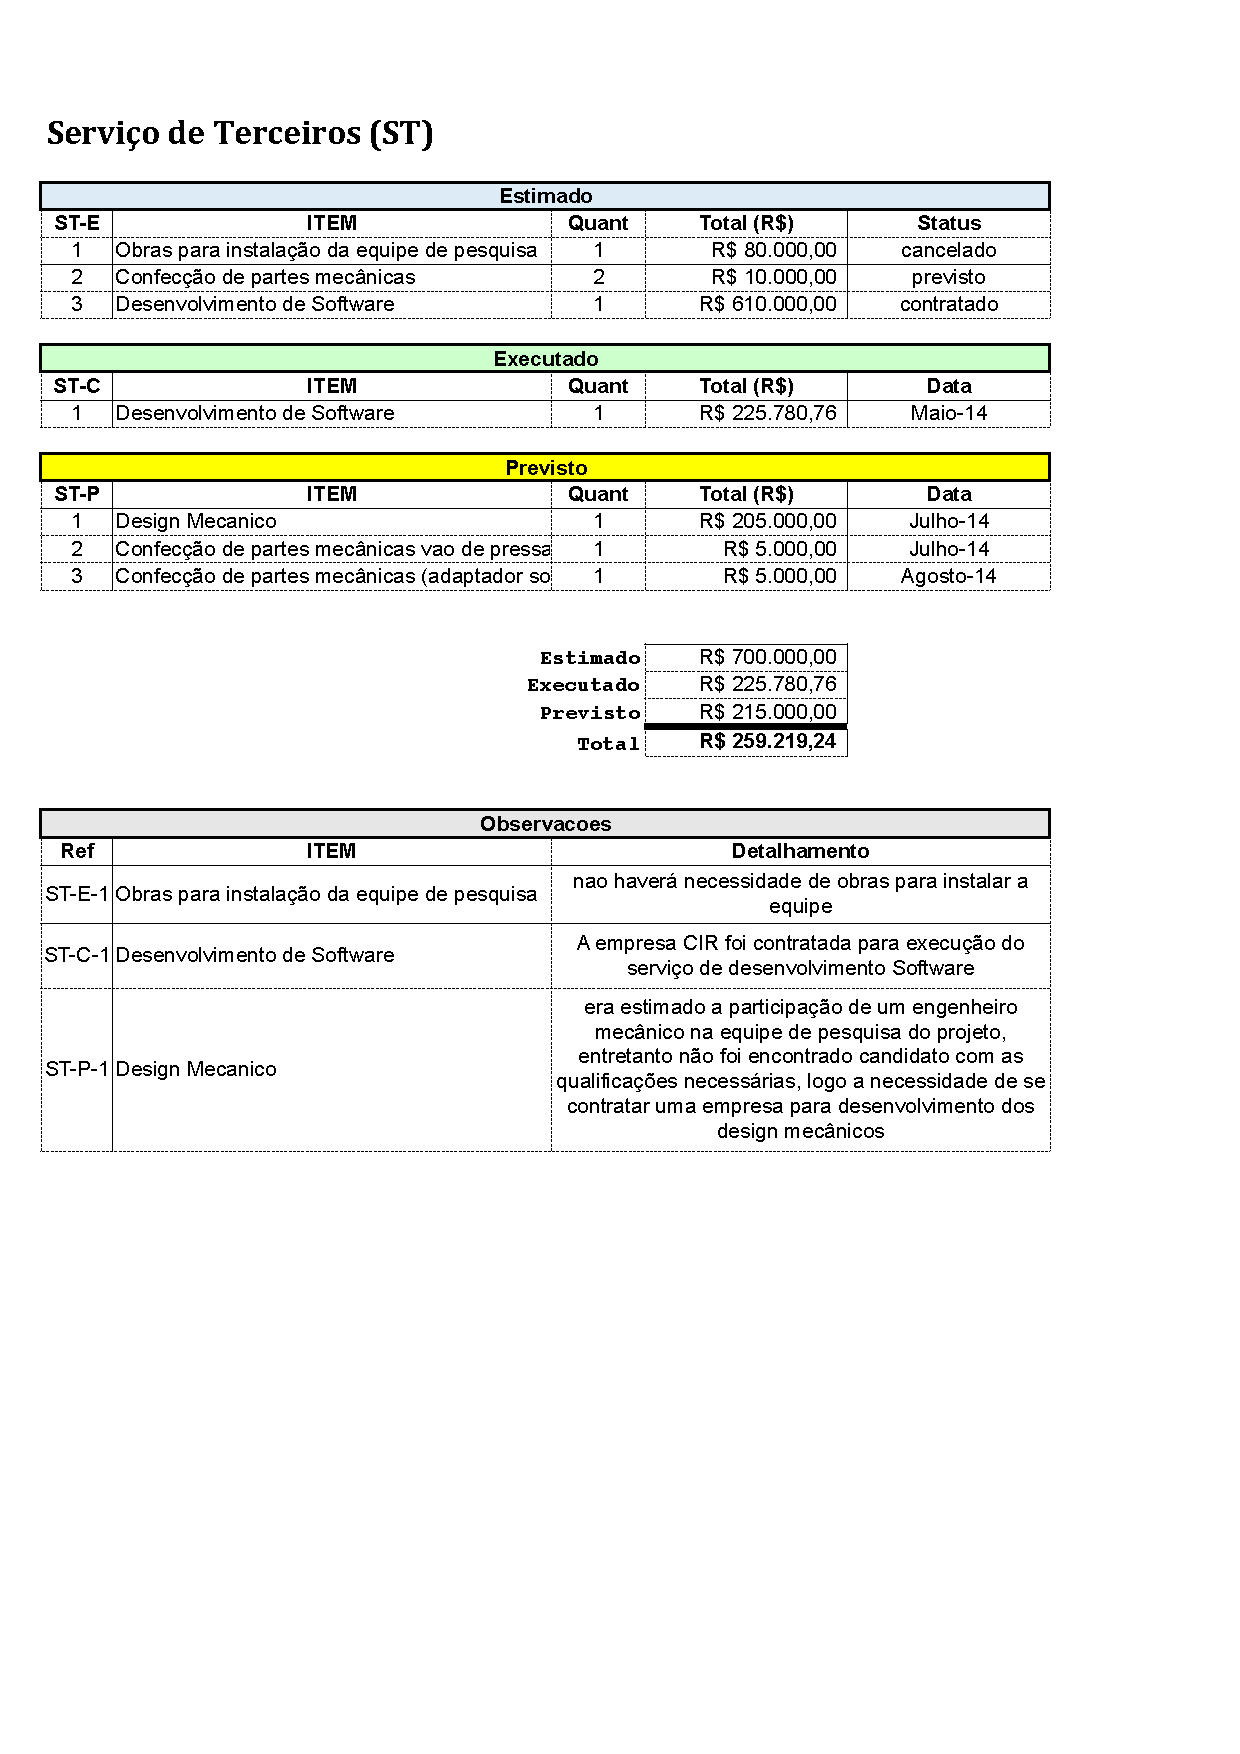
\includegraphics[width=1\columnwidth]{figs/financeiro/ROSA_Cronograma_Fisico_Financeiro_05_26_2014_ST.pdf}
\end{center}

\subsection{Material de consumo}

\begin{center}
  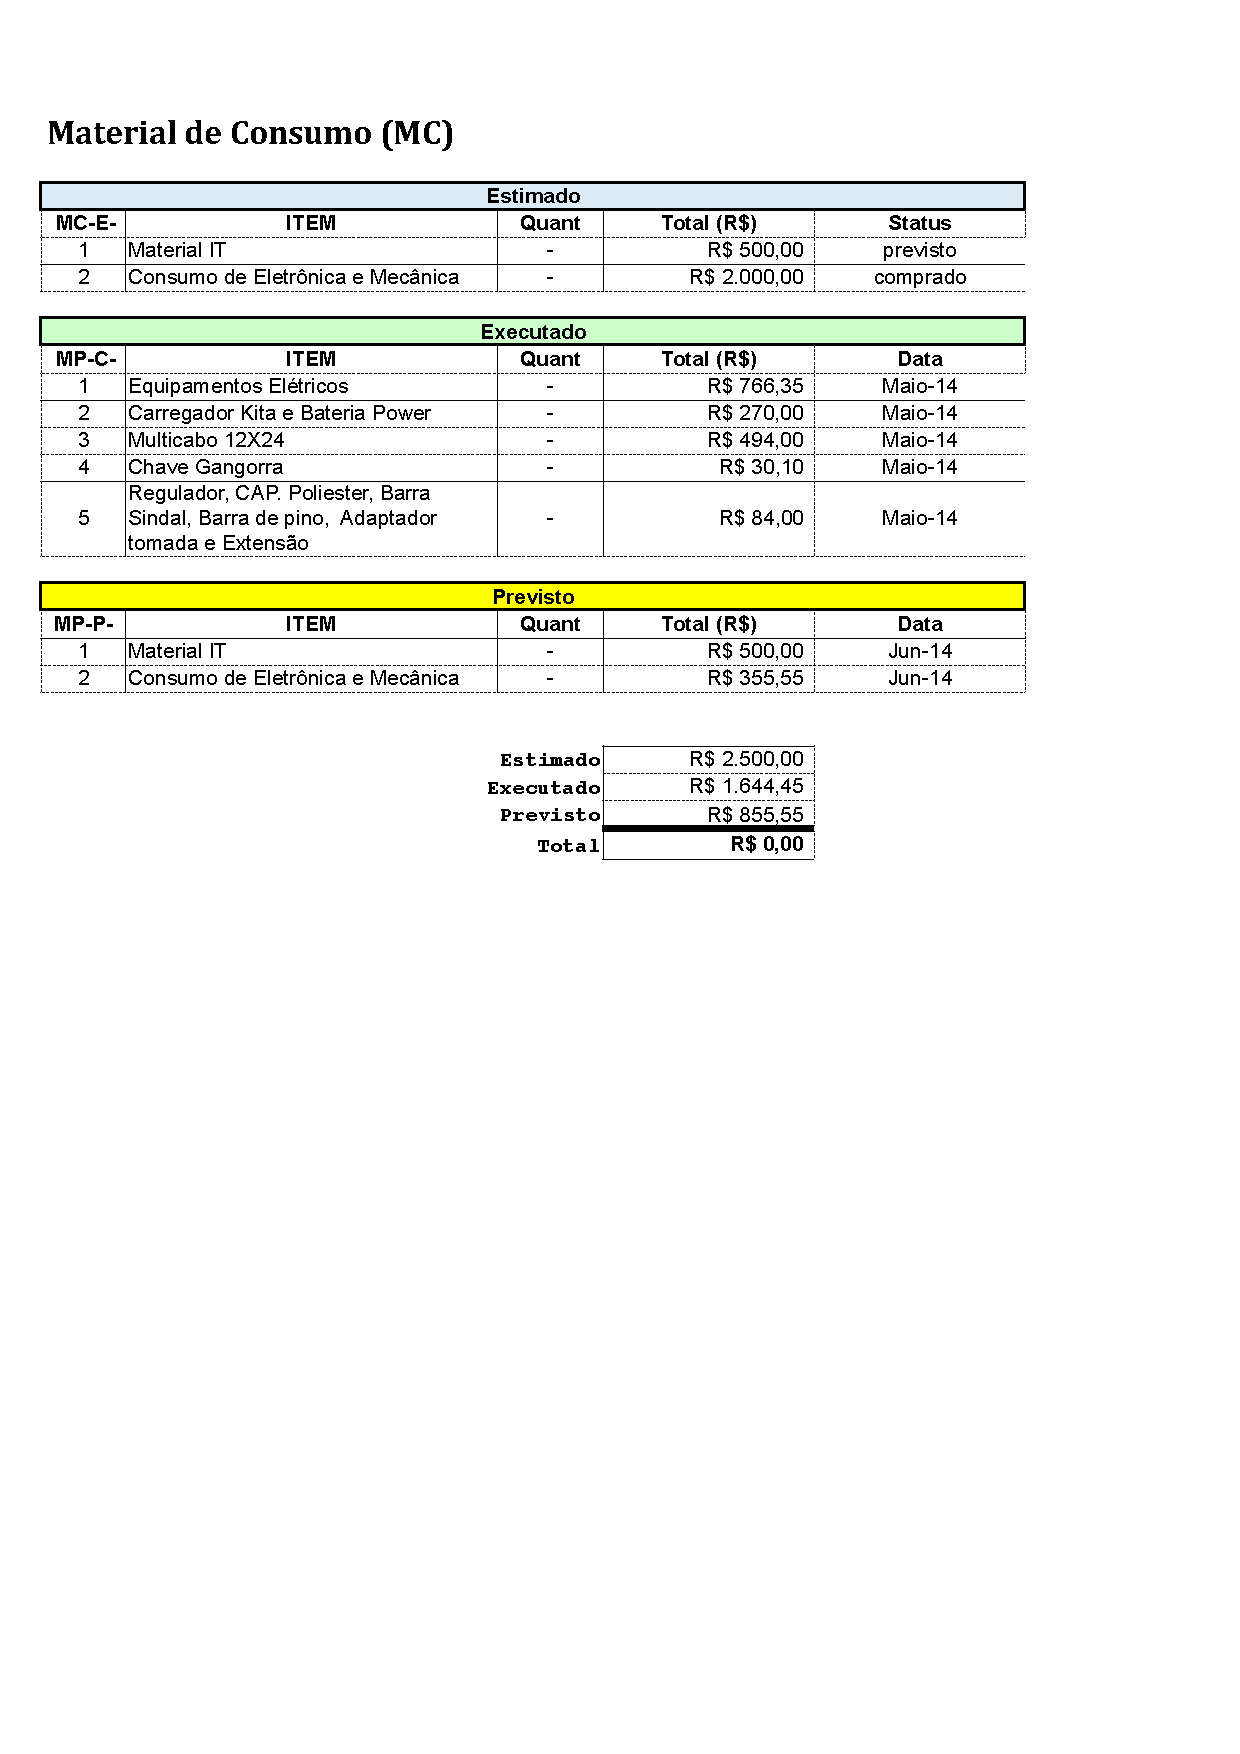
\includegraphics[width=1\columnwidth]{figs/financeiro/ROSA_Cronograma_Fisico_Financeiro_05_26_2014_MC.pdf}
\end{center}

\subsection{Material permanente}

\begin{center}
  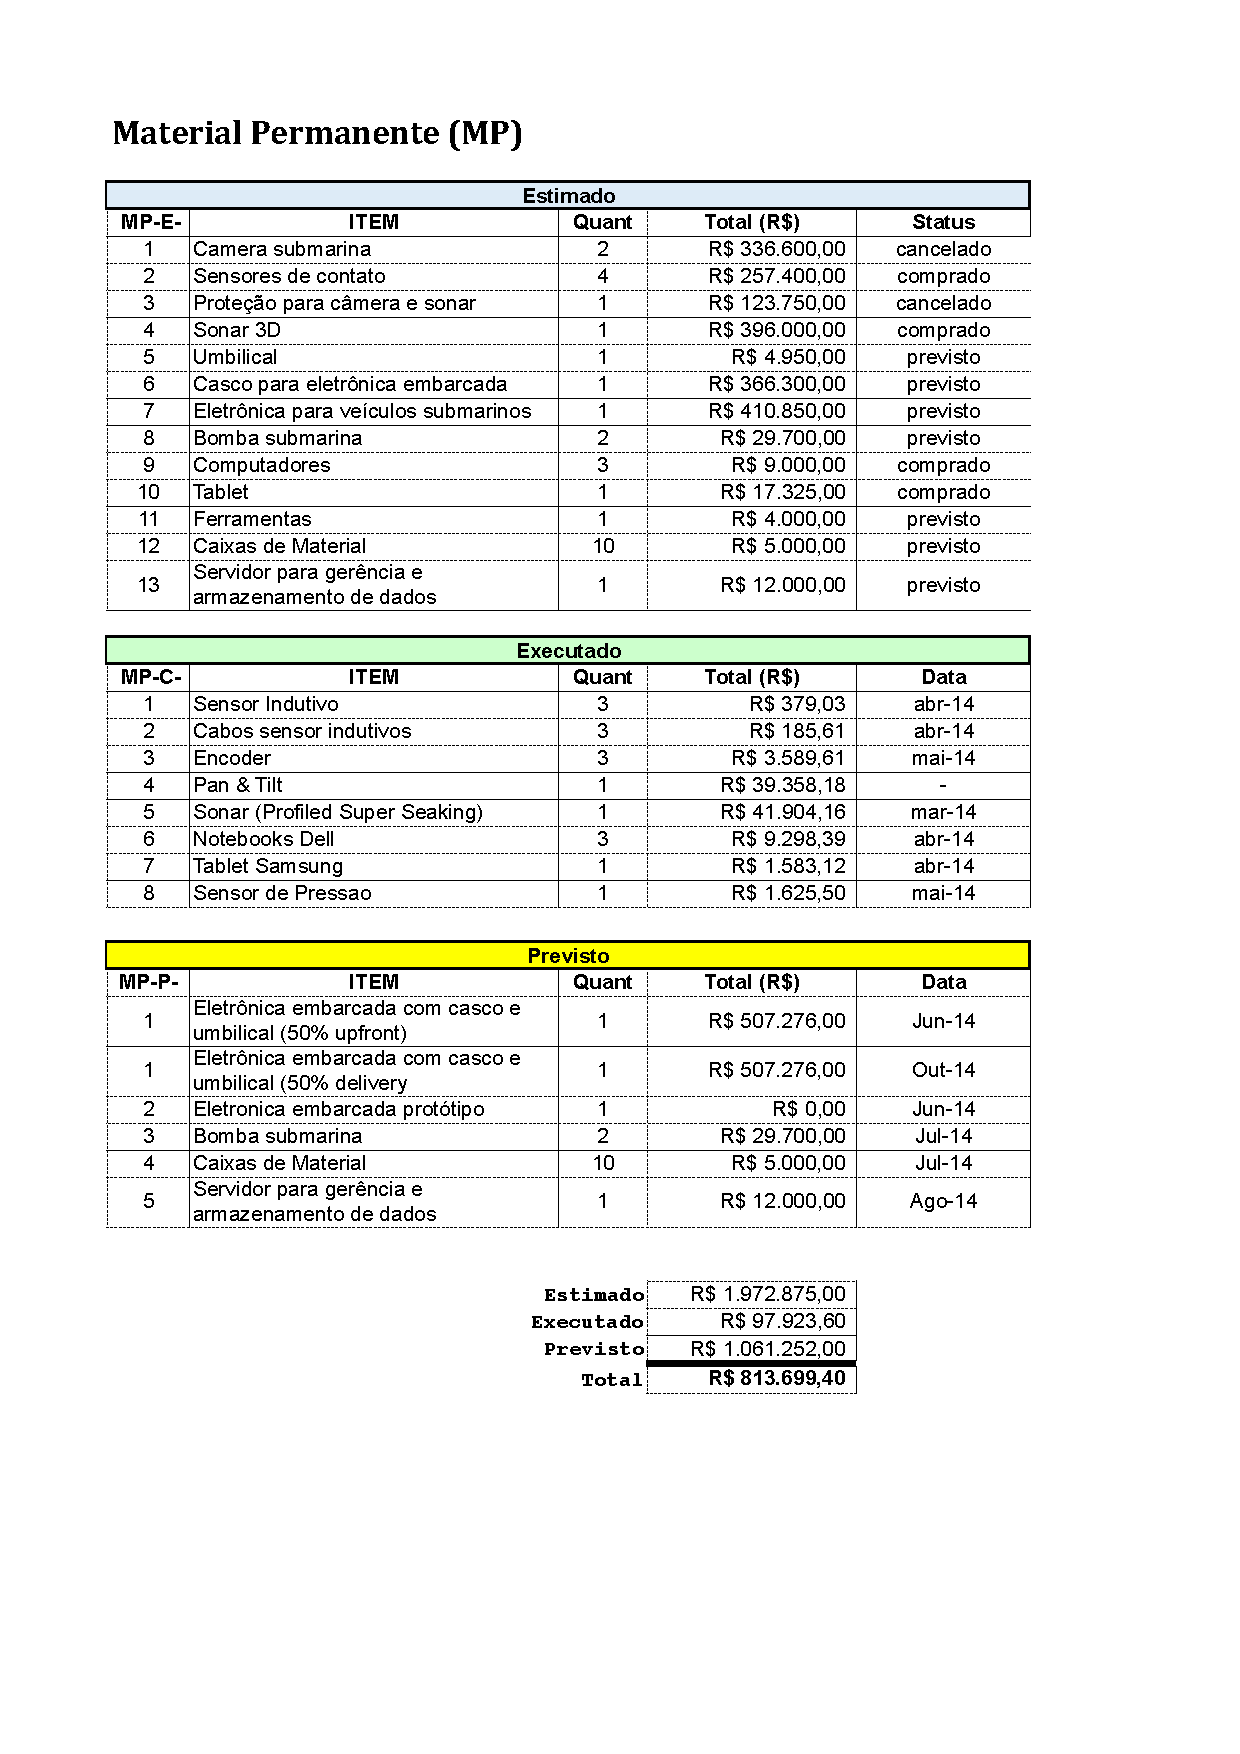
\includegraphics[width=1\columnwidth]{figs/financeiro/ROSA_Cronograma_Fisico_Financeiro_05_26_2014_MP.pdf}
\end{center}

\subsection{Viagens e di�rias}

\begin{center}
  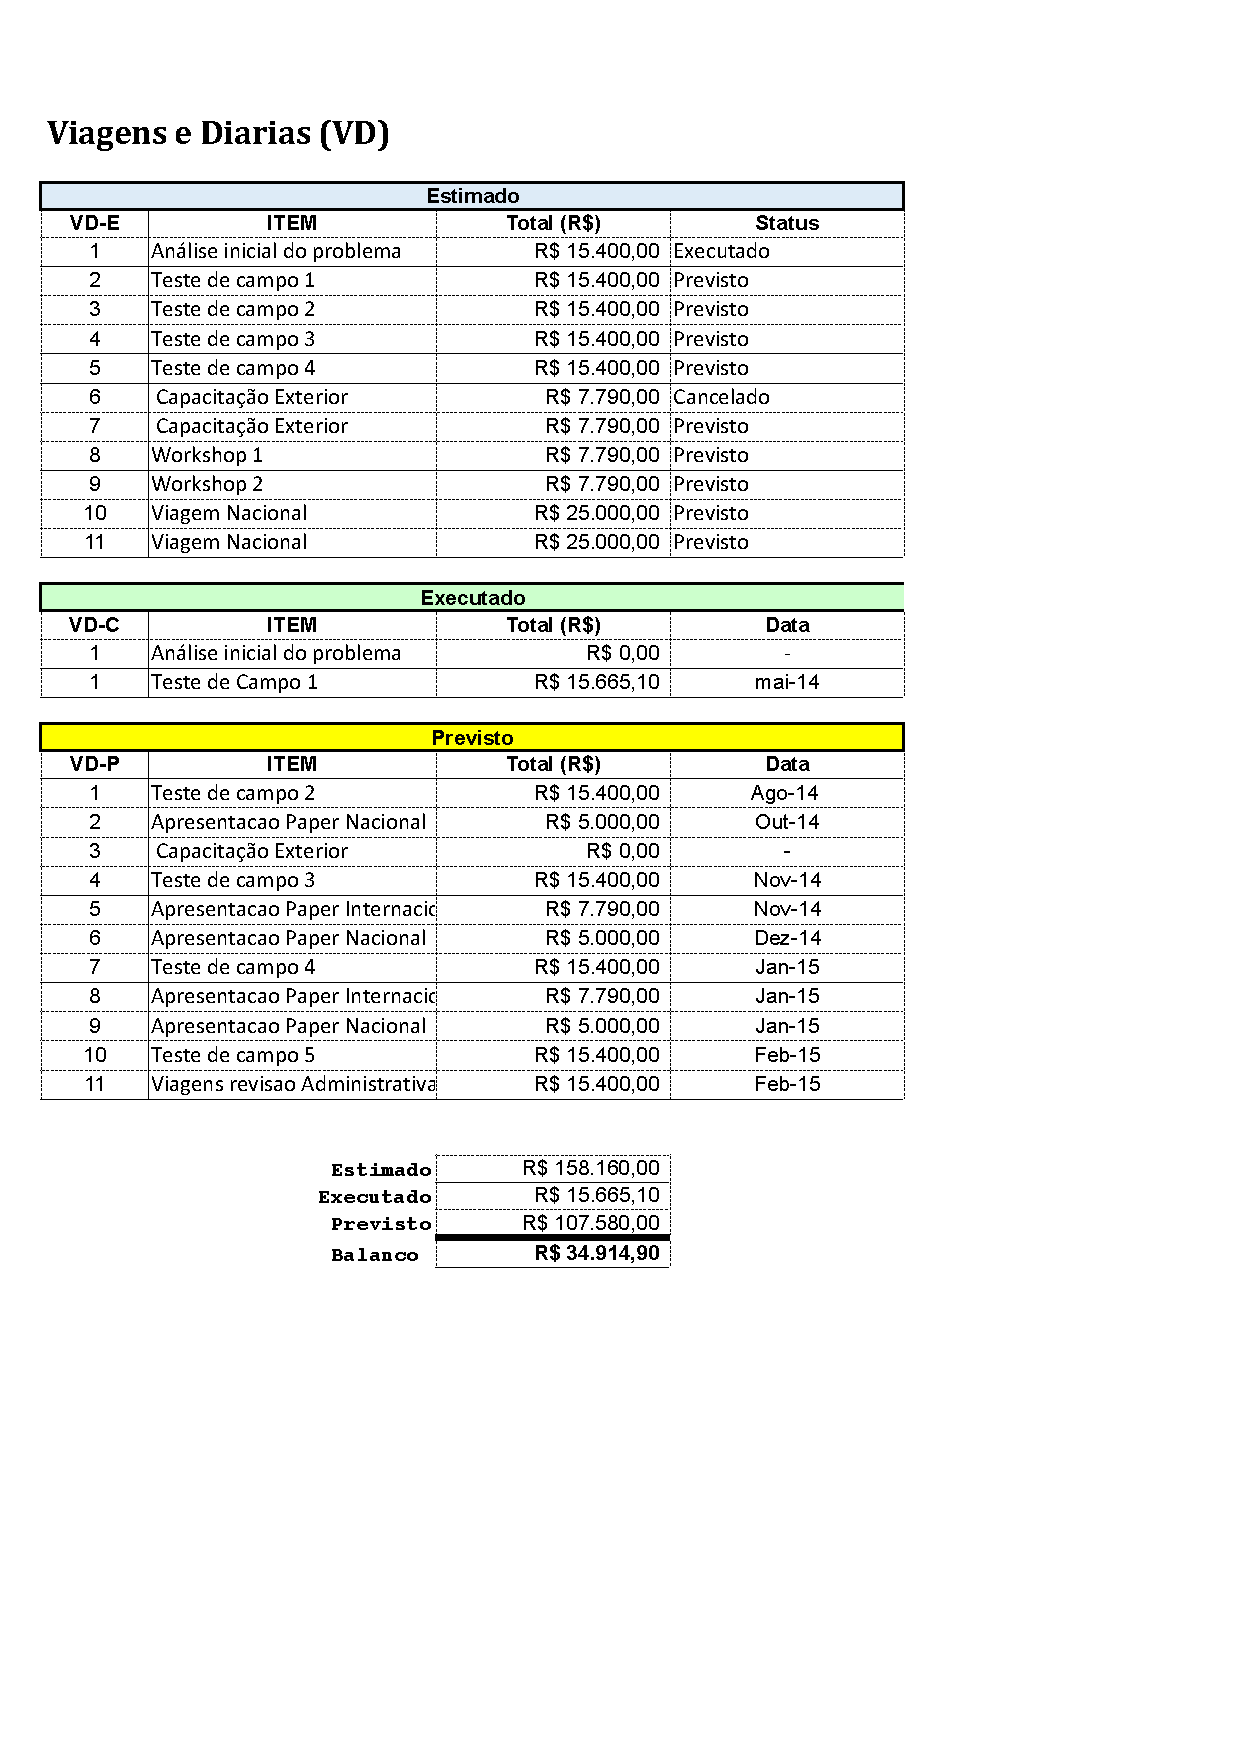
\includegraphics[width=1\columnwidth]{figs/financeiro/ROSA_Cronograma_Fisico_Financeiro_05_26_2014_VD.pdf}
\end{center}

\subsection{Outros}

\begin{center}
  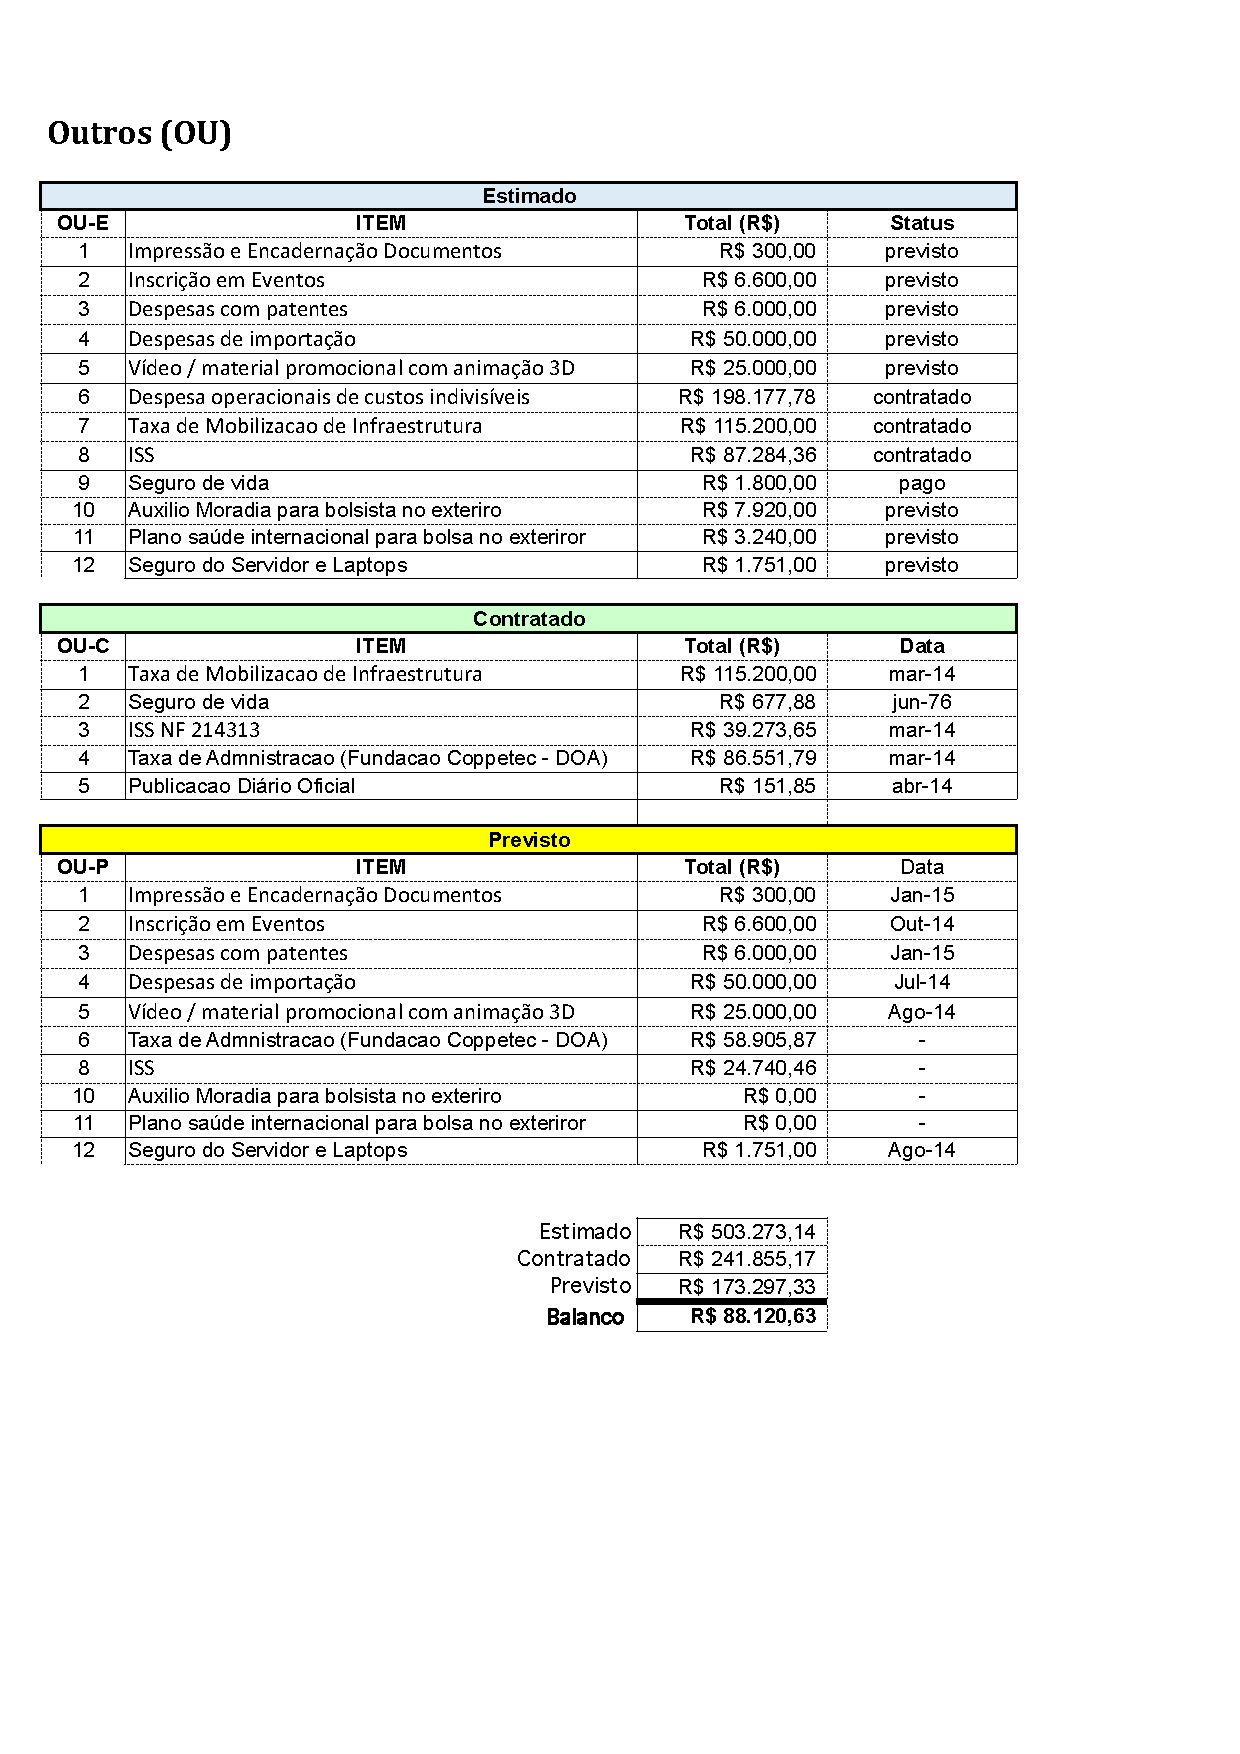
\includegraphics[width=1\columnwidth]{figs/financeiro/ROSA_Cronograma_Fisico_Financeiro_05_26_2014_Ou.pdf}
\end{center}

\subsection{Balan�o}

\begin{center}
  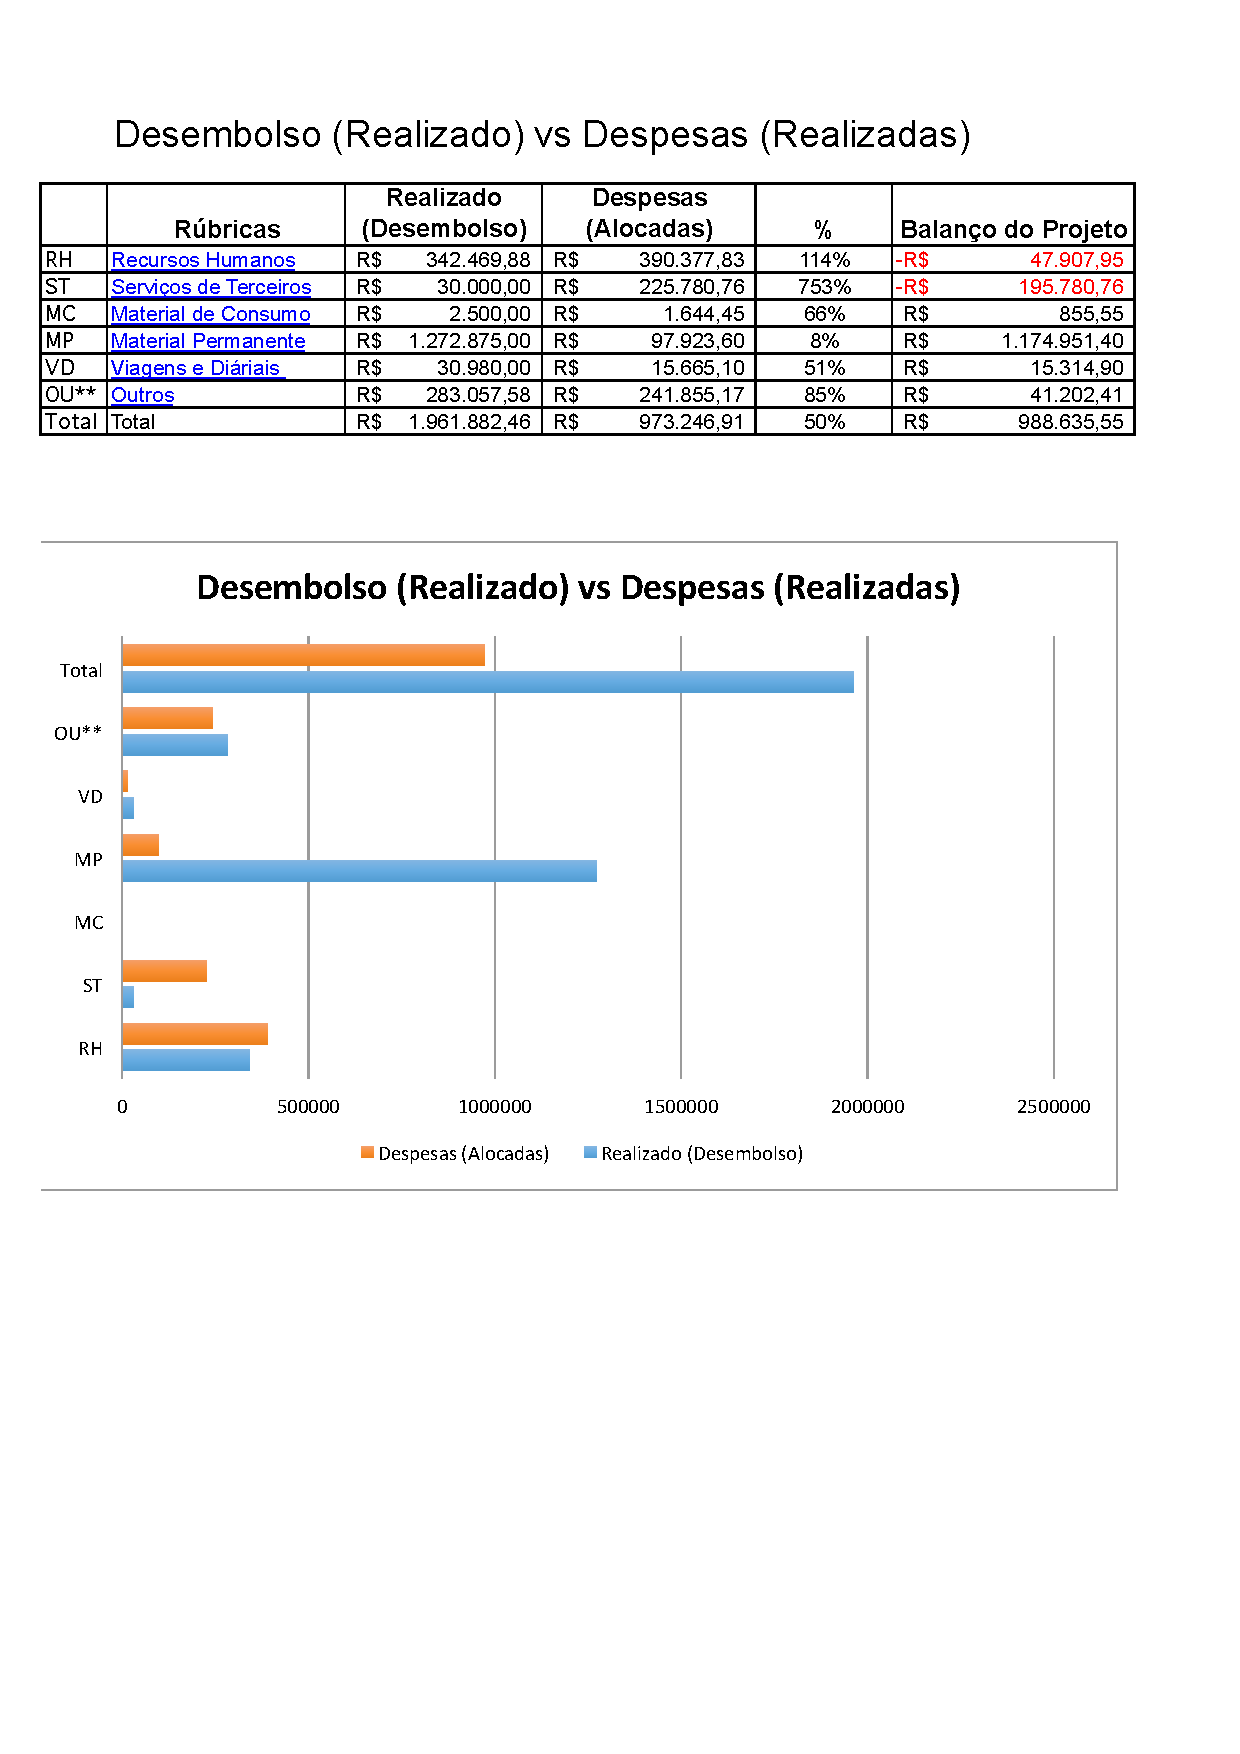
\includegraphics[width=1\columnwidth]{figs/financeiro/ROSA_Cronograma_Fisico_Financeiro_05_26_2014_Balanco.pdf}
\end{center}


\subsection{Cronograma}

\begin{center}
  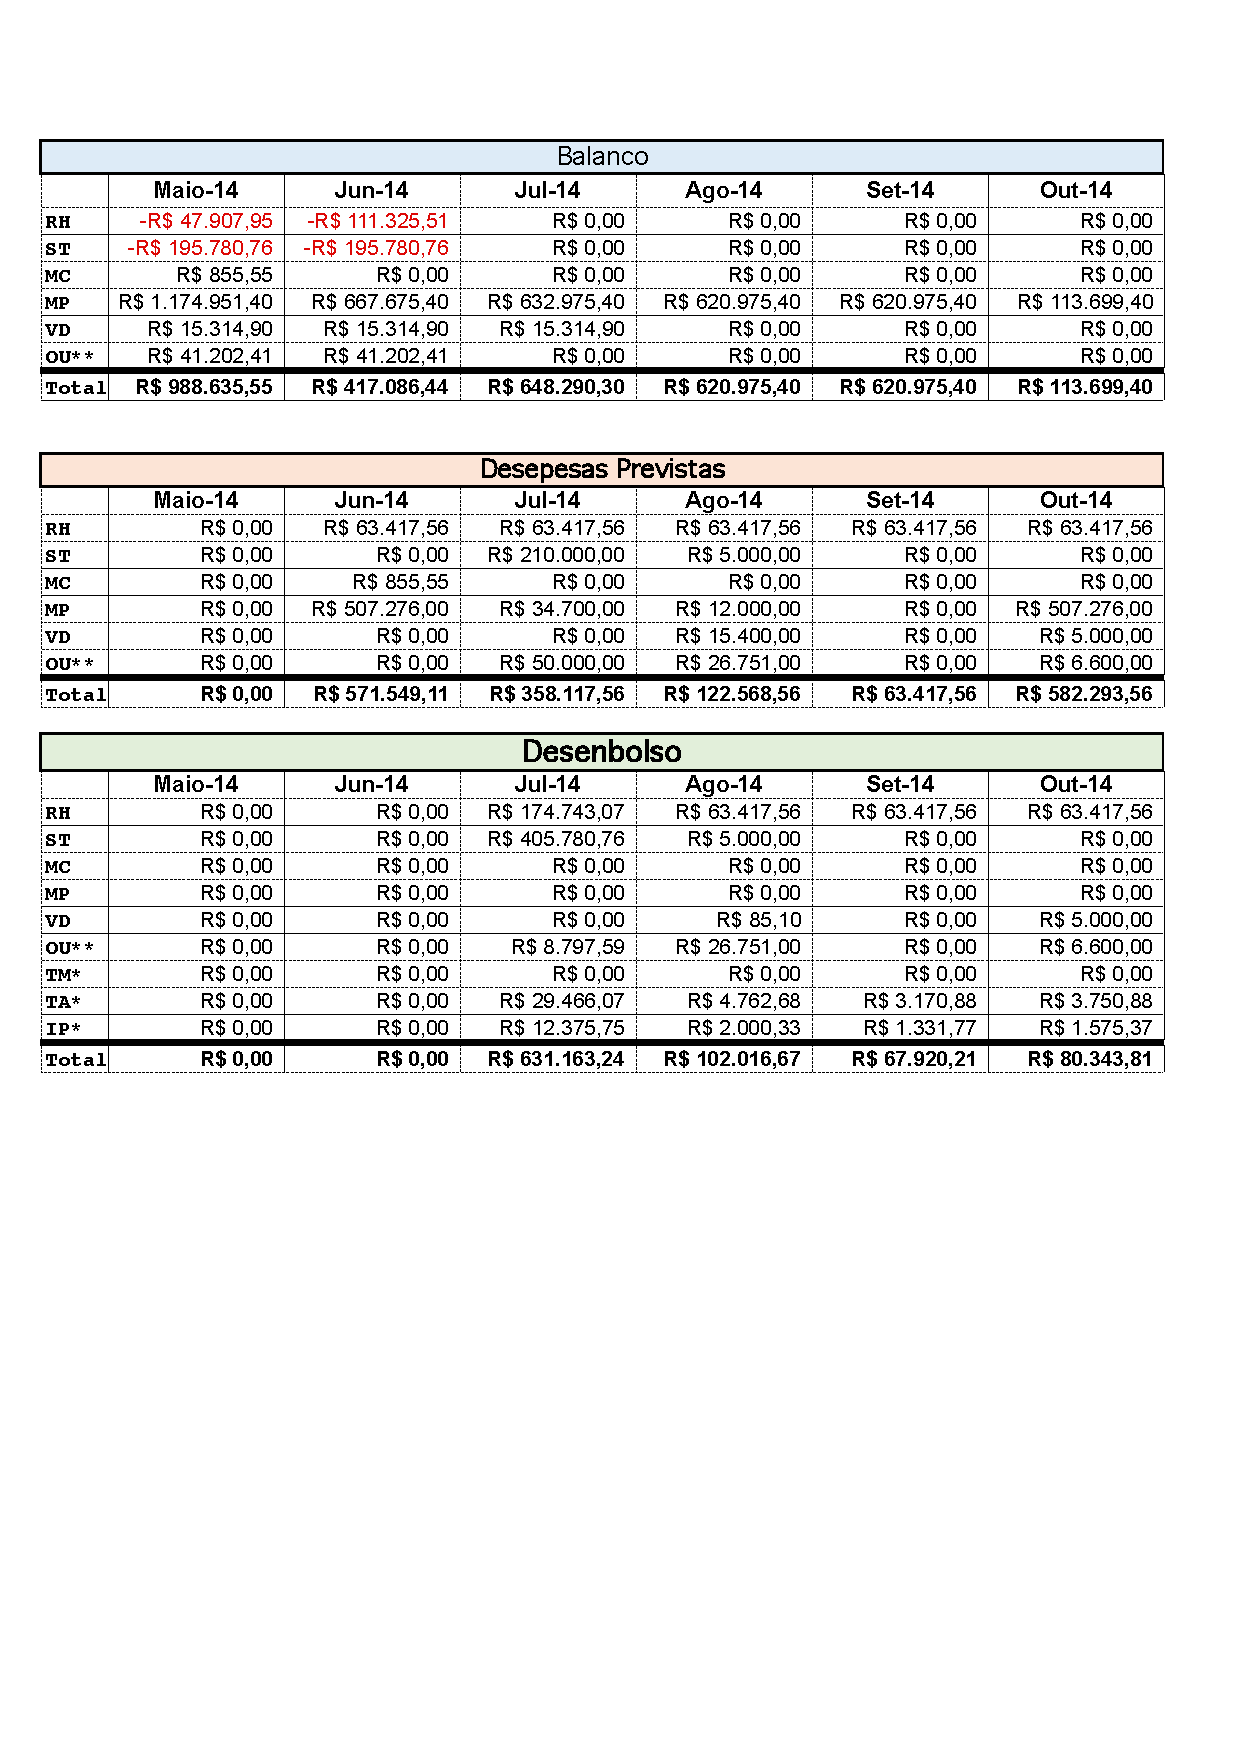
\includegraphics[width=1\columnwidth]{figs/financeiro/ROSA_Cronograma_Fisico_Financeiro_05_26_2014_Cronograma_Desenbolso.pdf}
\end{center}

\begin{center}
  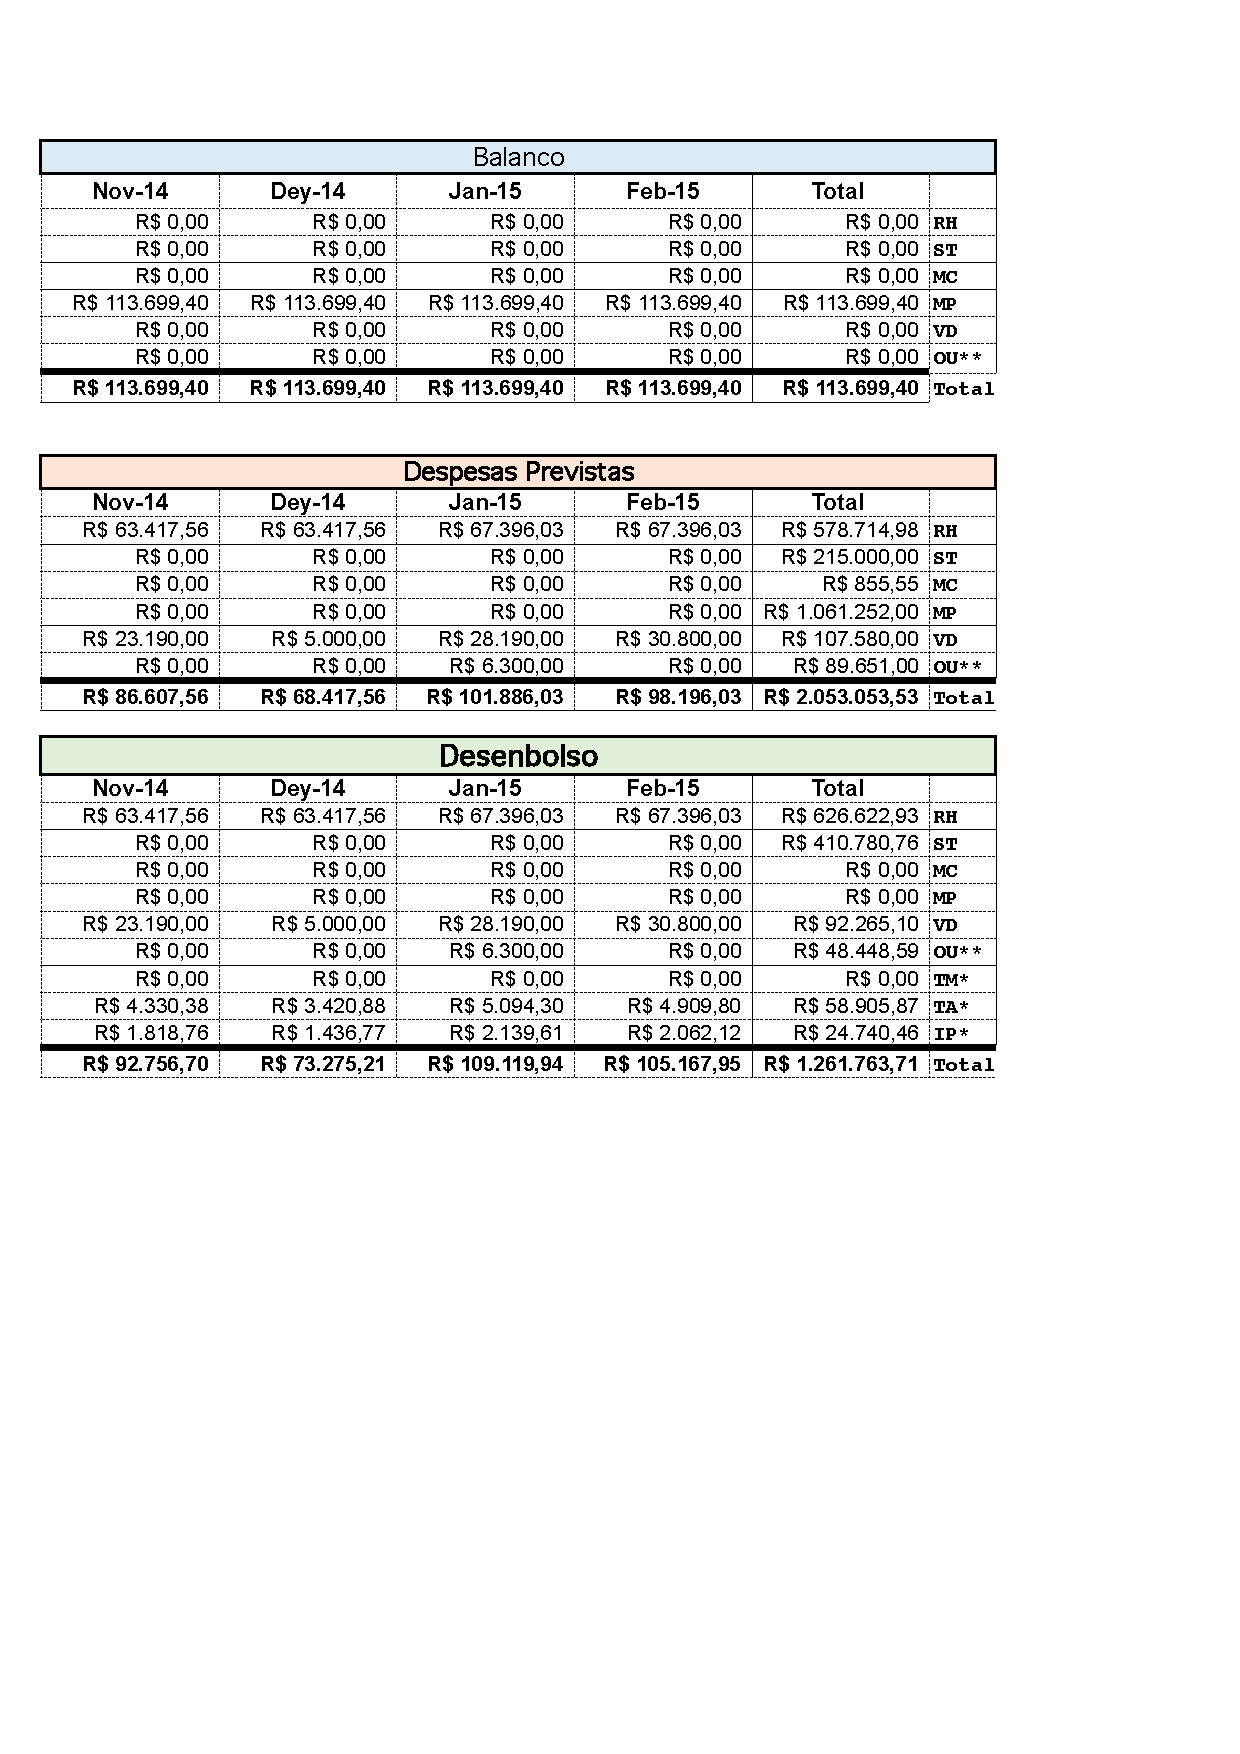
\includegraphics[width=1\columnwidth]{figs/financeiro/ROSA_Cronograma_Fisico_Financeiro_05_26_2014_Cronograma_Desenbolso_2.pdf}
\end{center}







